\section{微分的应用}

本节以曲率为例讲解微分的应用。

%============================================================
\subsection{弧微分和曲率}

在工程技术中,要经常考虑曲线的弯曲程度,所谓曲线的“曲率”。

\begin{figure}[h]
\centering
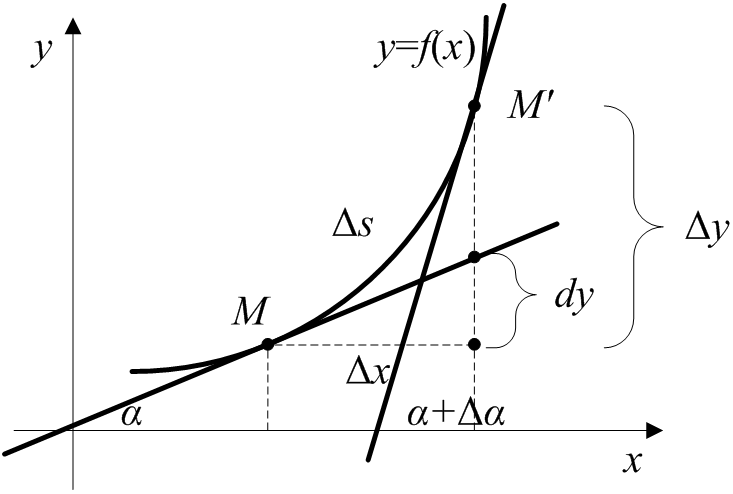
\includegraphics[height=4cm]{2.4.png}
\end{figure}

\begin{definition}[曲率]
我们定义曲线$y$上,切线转过的角度$\Delta \alpha $和弧长$\Delta s=\overset\frown{MM'}$的比值为{\bf 该弧段的平均曲率},记作$\bar{\kappa}$,即:
\[
\bar{\kappa}:=\frac{\Delta \alpha}{\Delta s}
\]
如果当$\Delta s\rightarrow 0$时$\bar{\kappa}$存在极限,就称该极限为{\bf 曲线$y$在点{\it M}处的曲率},记作$\kappa $,即:
\[
\kappa :=\underset{\Delta s\rightarrow 0}{\lim}\bar{\kappa}=\underset{\Delta s\rightarrow 0}{\lim}\frac{\Delta \alpha}{\Delta s}=\frac{d\alpha}{ds}
\]
\end{definition}

首先求解$d\alpha $:
\begin{align*}
&\because \frac{dy}{dx}=\tan \alpha \\
&\therefore \frac{d^2y}{dx^2}=\frac{d}{dx}\left( \tan \alpha \right) =\sec ^2\alpha \cdot \frac{d\alpha}{dx} \\
&\therefore d\alpha =\frac{d^2y}{dx^2}\cdot \frac{dx}{\sec ^2\alpha}=\frac{d^2y}{dx^2}\cdot \frac{dx}{1+\tan ^2\alpha}=\frac{d^2y}{dx^2}\cdot \frac{1}{1+\left( \frac{dy}{dx} \right) ^2}\cdot dx
\end{align*}
再求解$ds$(称为{\bf 弧微分}):
\[
ds=\sqrt{\left( dx \right) ^2+\left( dy \right) ^2}=\sqrt{1+\left( \frac{dy}{dx} \right) ^2}\cdot dx
\]
结合上述两式,得到曲率公式:
\[
\kappa =\underset{\Delta s\rightarrow 0}{\lim}\bar{\kappa}=\underset{\Delta s\rightarrow 0}{\lim}\frac{\Delta \alpha}{\Delta s}=\frac{d\alpha}{ds}=\frac{\frac{d^2y}{dx^2}\cdot \frac{1}{1+\left( \frac{dy}{dx} \right) ^2}\cdot dx}{\sqrt{1+\left( \frac{dy}{dx} \right) ^2}\cdot dx}=\frac{d^2y}{dx^2}\cdot \frac{1}{\left[ 1+\left( \frac{dy}{dx} \right) ^2 \right] ^{3/2}}
\]

\begin{tcolorbox}
曲率有正有负,表示凸还是凹。
其次,弧微分这个概念在微积分中会频繁出现,特别是在多元函数微积分中。
\end{tcolorbox}




